\documentclass{article}\usepackage[]{graphicx}\usepackage[]{color}
%% maxwidth is the original width if it is less than linewidth
%% otherwise use linewidth (to make sure the graphics do not exceed the margin)
\makeatletter
\def\maxwidth{ %
  \ifdim\Gin@nat@width>\linewidth
    \linewidth
  \else
    \Gin@nat@width
  \fi
}
\makeatother

\definecolor{fgcolor}{rgb}{0.345, 0.345, 0.345}
\newcommand{\hlnum}[1]{\textcolor[rgb]{0.686,0.059,0.569}{#1}}%
\newcommand{\hlstr}[1]{\textcolor[rgb]{0.192,0.494,0.8}{#1}}%
\newcommand{\hlcom}[1]{\textcolor[rgb]{0.678,0.584,0.686}{\textit{#1}}}%
\newcommand{\hlopt}[1]{\textcolor[rgb]{0,0,0}{#1}}%
\newcommand{\hlstd}[1]{\textcolor[rgb]{0.345,0.345,0.345}{#1}}%
\newcommand{\hlkwa}[1]{\textcolor[rgb]{0.161,0.373,0.58}{\textbf{#1}}}%
\newcommand{\hlkwb}[1]{\textcolor[rgb]{0.69,0.353,0.396}{#1}}%
\newcommand{\hlkwc}[1]{\textcolor[rgb]{0.333,0.667,0.333}{#1}}%
\newcommand{\hlkwd}[1]{\textcolor[rgb]{0.737,0.353,0.396}{\textbf{#1}}}%

\usepackage{framed}
\makeatletter
\newenvironment{kframe}{%
 \def\at@end@of@kframe{}%
 \ifinner\ifhmode%
  \def\at@end@of@kframe{\end{minipage}}%
  \begin{minipage}{\columnwidth}%
 \fi\fi%
 \def\FrameCommand##1{\hskip\@totalleftmargin \hskip-\fboxsep
 \colorbox{shadecolor}{##1}\hskip-\fboxsep
     % There is no \\@totalrightmargin, so:
     \hskip-\linewidth \hskip-\@totalleftmargin \hskip\columnwidth}%
 \MakeFramed {\advance\hsize-\width
   \@totalleftmargin\z@ \linewidth\hsize
   \@setminipage}}%
 {\par\unskip\endMakeFramed%
 \at@end@of@kframe}
\makeatother

\definecolor{shadecolor}{rgb}{.97, .97, .97}
\definecolor{messagecolor}{rgb}{0, 0, 0}
\definecolor{warningcolor}{rgb}{1, 0, 1}
\definecolor{errorcolor}{rgb}{1, 0, 0}
\newenvironment{knitrout}{}{} % an empty environment to be redefined in TeX

\usepackage{alltt}


\usepackage{graphicx}
\graphicspath{ {TwitterSentiment/} }
\IfFileExists{upquote.sty}{\usepackage{upquote}}{}
\begin{document}

\title {Comparison of Stock Price vs Twitter Sentiment} 
\author { Paul Wagner  
\\ School of Information Technology 
\\ Illinois State University
\\
\texttt{pgwagne@ilstu.edu}}
\date{\today} 
\maketitle

Twitter sentiment, which was used in my graph looked at general sentiment of 200 stocks that contained the Walmart ticker symbol of WMT that was then divided by 100. The change in stock price that I used was the stock price subtracted from \$85.

There appears to be a correlation between general twitter sentiment and stock price. For 4 out of the 5 days during the week of Dec 1st through 5th, positive or negative Twitter sentiment corresponded to the day’s stock price movement. 

The only exception to the general correspondence between stock price and Twitter sentiment was Thursday, Dec 4th in which Tweets regarding WMT were positive while the day’s overall movement was negative. This was likely due to a positive spike in stock price during the intraday trading on the 4th in which the stock jumped over a point but still wasn’t able to make up the loss incurred during overnight trading during Dec 3rd and 4th in which it lost nearly a point and a half from its high on the 3rd.

Sentiment dropped sharply on Dec 3rd and 4th likely in response to UBS’s announcement that they had downgraded WMT from a Buy to Neutral. Shares have climbed by 11\% over the last month due to lower gas prices, good holiday sales and overall market momentum. Analysts believe that WMT is approaching is high end of its price potential and are taking earnings.


\begin{knitrout}
\definecolor{shadecolor}{rgb}{0.969, 0.969, 0.969}\color{fgcolor}
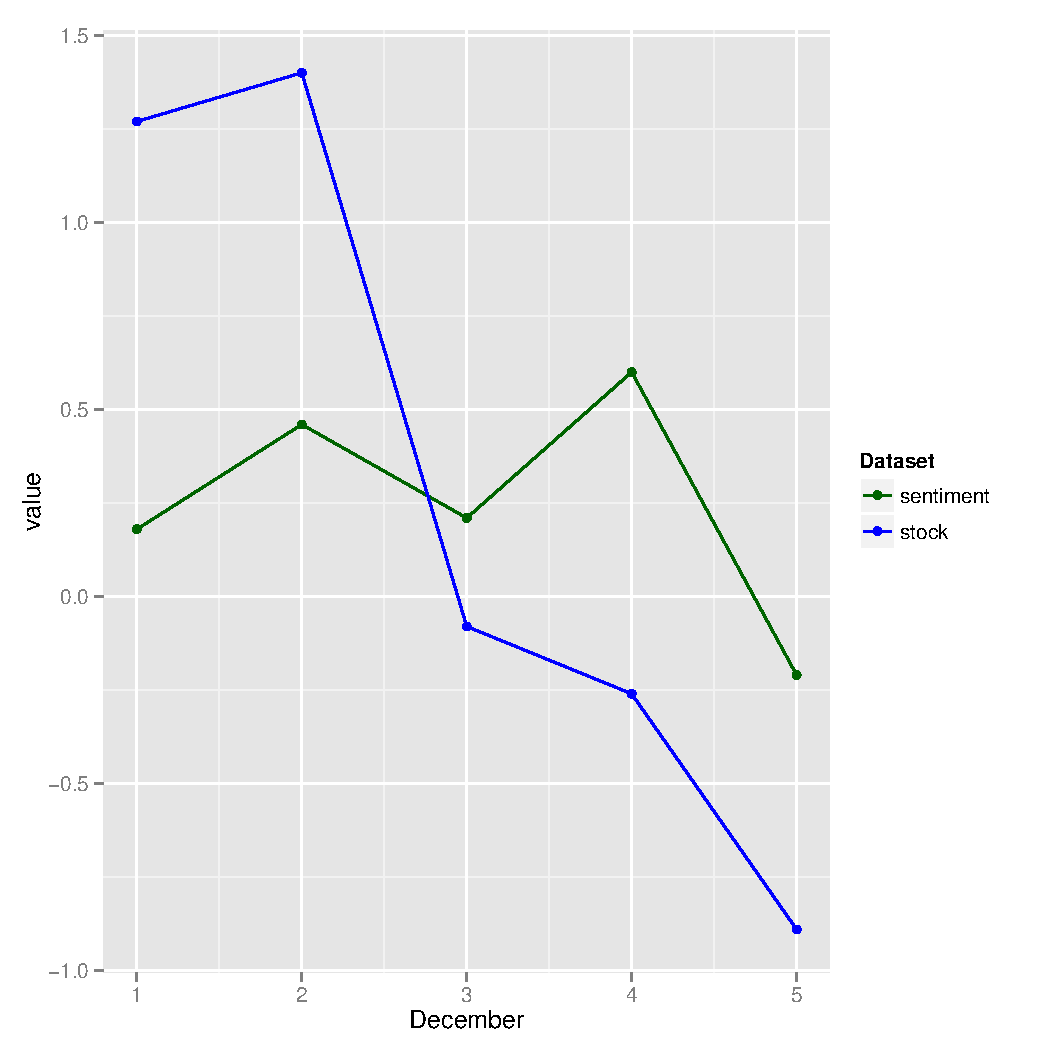
\includegraphics[width=\maxwidth]{figure/unnamed-chunk-1-1} 

\end{knitrout}


\begin{figure}[h!]
\caption{Twitter Sentiment for December 1st.}
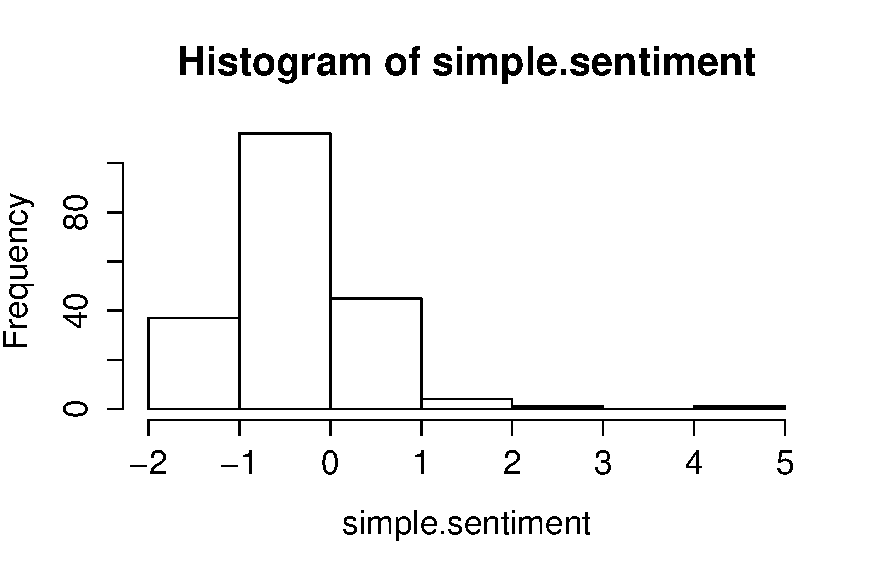
\includegraphics[width=6cm]{12-1.pdf}
\centering
\end{figure}

\begin{figure}[h!]
\caption{Twitter Sentiment for December 2nd.}
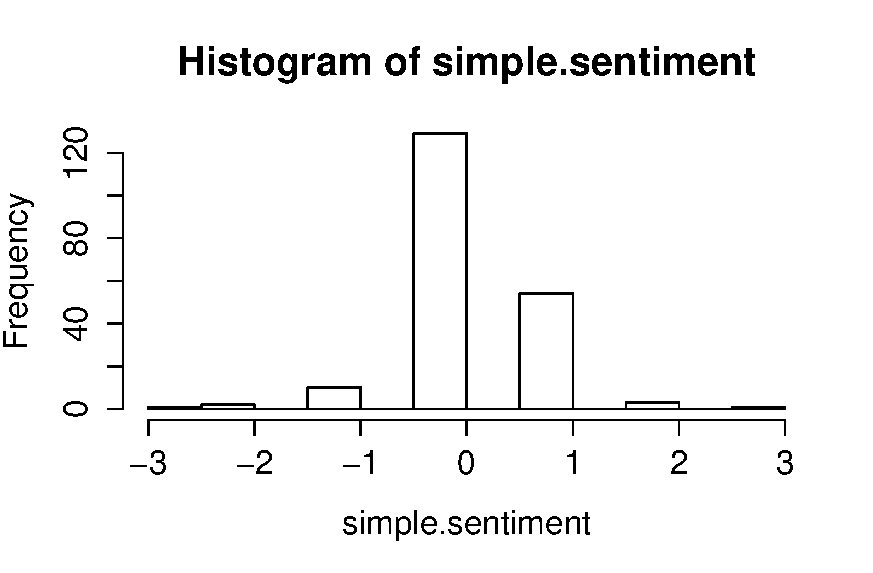
\includegraphics[width=6cm]{12-2.pdf}
\centering
\end{figure}

\begin{figure}[h!]
\caption{Twitter Sentiment for December 3rd.}
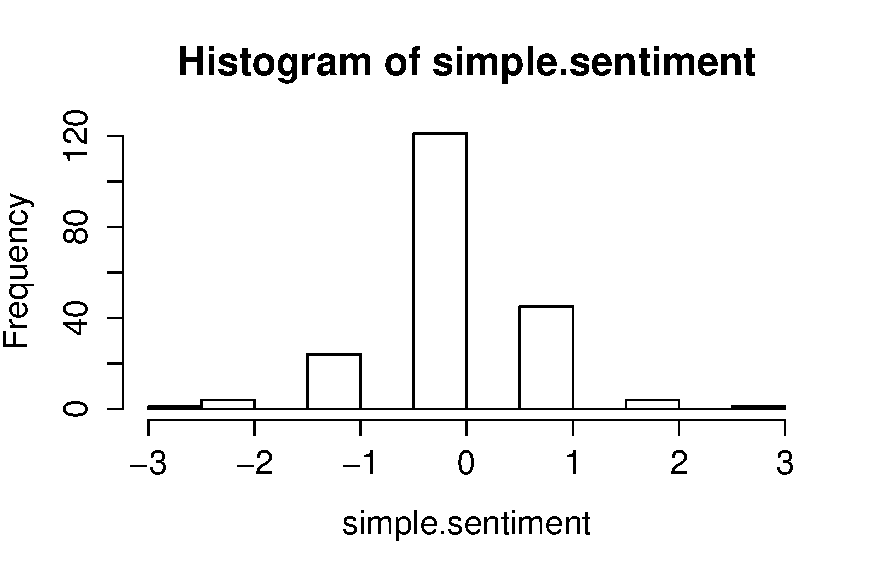
\includegraphics[width=6cm]{12-3.pdf}
\centering
\end{figure}

\begin{figure}[h!]
\caption{Twitter Sentiment for December 4th.}
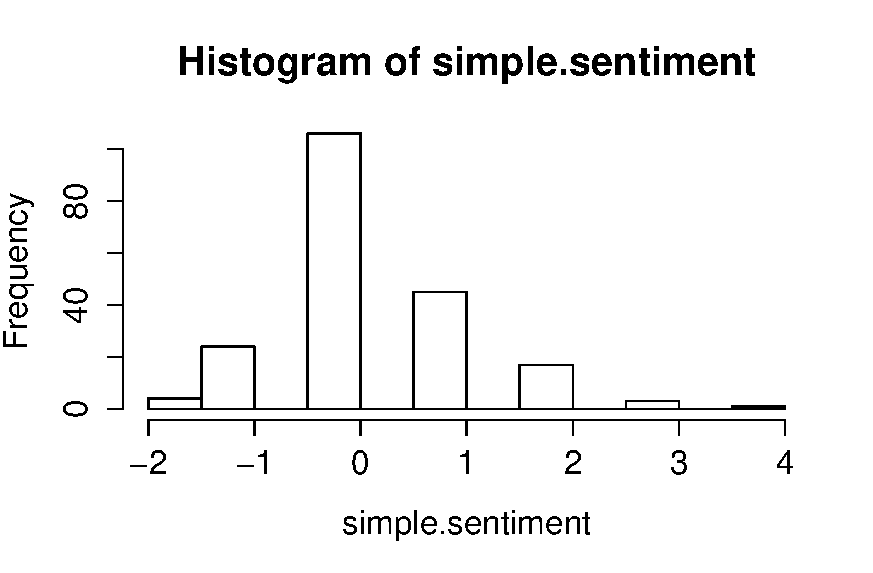
\includegraphics[width=6cm]{12-4.pdf}
\centering
\end{figure}

\begin{figure}[H!]
\caption{Twitter Sentiment for December 5th.}
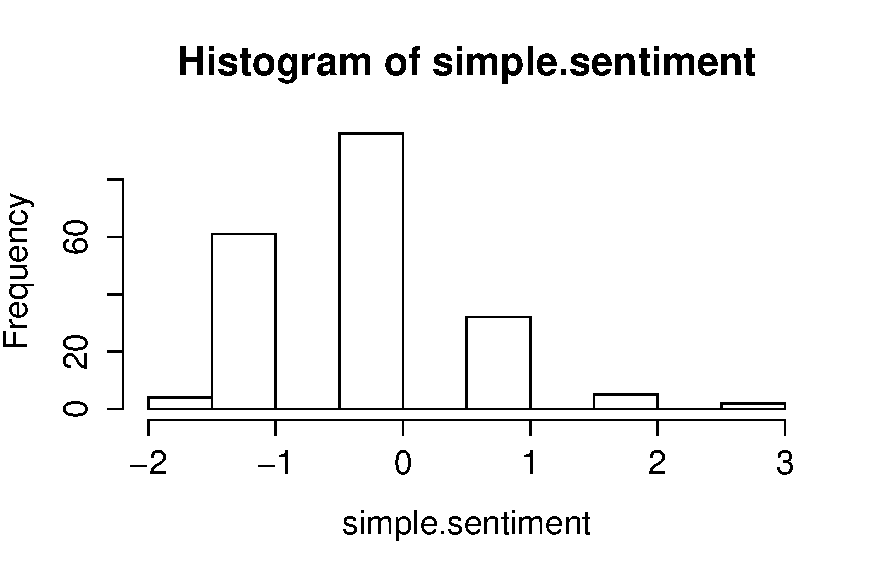
\includegraphics[width=6cm]{12-5.pdf}
\centering
\end{figure}
 





\end{document}
